\documentclass[12pt,
border=1pt]{standalone}
\usepackage{pgfplots}
\usepackage{amsmath}
\usepackage{amssymb}

\pgfplotsset{compat=newest,
	width=6cm, height=5cm,
	xtick pos=left, ytick pos=left,
	%            scaled x ticks=real:1e-6,
}
% Kernel 2 FP64
\begin{document}
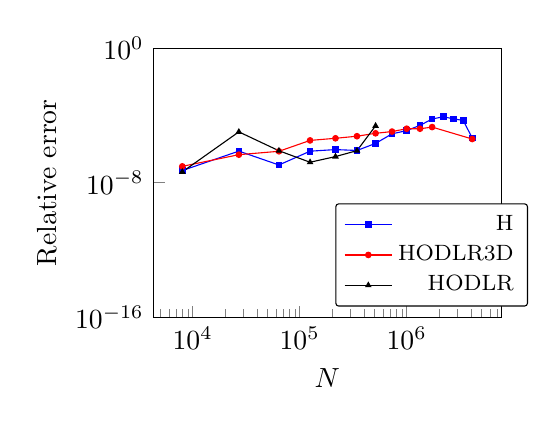
\begin{tikzpicture}[every mark/.append style={mark size=1pt}]
	\begin{axis}[xlabel={$N$},
	ylabel={Relative error},
%		legend pos=south east,
		legend style={
                at={(0.8,0.04)},
               anchor=south,
               legend columns=1,
               cells={anchor=east},
              font=\footnotesize,
               rounded corners=1pt,
               },
		xmode = log,
	    ymode = log,
	   % xmin = 1e3,
	   % xmax = 1e6,
	    ymin = 1e-16,
	    ymax = 1e-0,
	   % xtick={1e-10, 1e-8, 1e-6,  1e-4,  1e-2},
	   % ytick={1e-8, 1e-6,  1e-4,  1e-2, 1e-0}
		]
		
		\addplot[
		color=blue,
		mark=square*,
		] coordinates {
(8000,5.307450e-08)
(27000,7.596810e-07)
(64000,1.137690e-07)
(125000,7.521850e-07)
(216000,9.368660e-07)
(343000,8.278650e-07)
(512000,2.182760e-06)
(729000,8.070650e-06)
(1000000,1.259530e-05)
(1331000,2.574730e-05)
(1728000,6.146410e-05)
(2197000,8.353590e-05)
(2744000,6.280750e-05)
(3375000,5.040420e-05)
(4096000,4.532280e-06)
% (4913000,9.745900e-06)
% (5832000,9.030440e-06)
% (6859000,4.321330e-06)
		};
		\addplot[
		color=red,
		mark=*,
		] coordinates {
(8000,9.439170e-08)
(27000,4.660330e-07)
(64000,7.414970e-07)
(125000,3.284480e-06)
(216000,4.389440e-06)
(343000,5.836740e-06)
(512000,8.697790e-06)
(729000,1.101590e-05)
(1000000,1.629840e-05)
(1331000,1.623180e-05)
(1728000,2.034470e-05)
(4096000,3.981880e-06)
		};
\addplot[
		color=black,
		mark=triangle*,
		] coordinates {
(8000,4.430180e-08)
(27000,1.057320e-05)
(64000,7.974380e-07)
(125000,1.653310e-07)
(216000,3.592410e-07)
(343000,8.092150e-07)
(512000,2.406340e-05)
		};
		\legend{H, HODLR3D, HODLR}	\end{axis}
\end{tikzpicture}
\end{document}